\documentclass{article}

\usepackage[utf8]{inputenc}
\usepackage{amsmath}
\usepackage{mathtools}
\usepackage{float}
\usepackage[english,noabbrev]{cleveref}

\DeclarePairedDelimiter{\ceil}{\lceil}{\rceil}
\DeclarePairedDelimiter\set\{\}

\begin{document}
	\section{Hypergraph representation}
	An undirected hypergraph $H=\left( V,E,c,\omega \right)$ with vertices $V=\set{ v_s \mid \textit{s site of MSA}}$ and hyperedges $E=\set{
		\set{
			v_s \mid v_s\ in\ repeat\ class\ r
		} \mid r\ repeat\ class \in RCCP
	}$, which connect exactly the vertices that represent sites of the repeat class of the hyperedge, describes the graph representation of the repeat class count problem \textit{RCCP} for a multiple sequence alignment \textit{MSA}. If a repeat class contains only one site, it creates a hyperedge $e \in E$ with $|e|=1$. The weights satisfy  $\forall v \in V: c\left(v\right)=1$ for vertices and $\forall e \in E: \omega\left(e\right)=1$ for hyperedges respectively.
	
	$H$ is now partitioned into $k$ blocks (\textit{k} is the number of CPU cores) according to a \textit{k-way partition}, which is defined by $\Pi = \set{V_1,...,V_k}$ with $\bigcup\nolimits_{i=1}^k, V_i \ne 0$ for $1 \leq i \leq k$ and $V_i \cap V_j = \emptyset$ for $i \neq j$.
	
	To divide as little repeat classes as possible we minimize the \textit{connectivity metric} described by  \[ \left(\lambda-1\right)\left(\Pi\right):=\sum\nolimits_{e \in E'}\left(\lambda\left(e\right)-1\right)\omega\left(e\right) = \sum\nolimits_{e \in E'}\left(\lambda\left(e\right)-1\right) \] with $\lambda\left(e\right):=|\Lambda\left(e\right)|$, $\Lambda\left(e\right):=\set{V_i \mid V_i \cap e = \emptyset}$ and the set of divided nets $E'$. 
	
	To preserve the \textit{Balancing} between blocks, we balance by the edge weights per block using the \textit{capacity constraint} \[ \left|\bigcap_{v \in V_i}I\left(v\right)\right| \leq \left(1+\epsilon\right)\frac{\left|E\right|}{k} \] with $I(v):=\set{\textit{nets incident towards v}}$.
	
	\begin{figure}[ht]
		\centering
		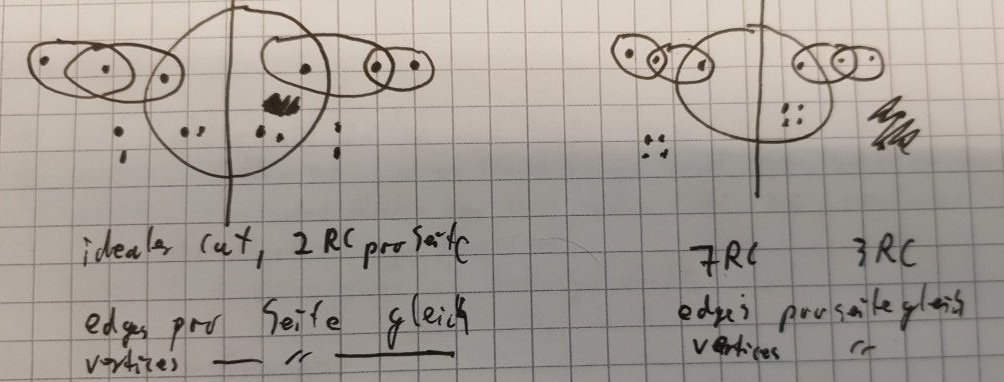
\includegraphics[width=0.65\textwidth]{example.png}
		\caption{Example for a problem with the vertex weight balancing}
		\label{fig:example}
	\end{figure}
	
	This only works, if KaHyPar allows for hyperedges with a single vertex (as described above). If this is not allowed, we additionally need to use the \textit{repeat class balancing constraint}: \[ \forall V_i \in \Pi: \left|\bigcap_{v \in V_i}I\left(v\right)\right| + \left|\set{v | v \in V_i \land I\left(v\right)=\emptyset}\right| \]
	
	The \textit{vertex balancing constraint} proposed by the practical explenation would not work because it treats vertices in a cut hyperedge equally to vertices without a hyperedge. This can cause problems with balancing as seen in \cref{fig:example}. However, this is an approximation because it will remove repeat classes as shown in \cref{fig:missingrc}.
	
	\begin{figure}[ht]
		\centering
		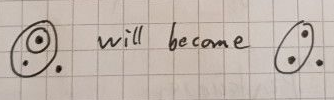
\includegraphics[width=0.65\textwidth]{missingrc.png}
		\caption{Missing repeat classes when using the repeat class balancing constraint}
		\label{fig:missingrc}
	\end{figure}
\end{document}